% move all configuration stuff into includes file so we can focus on the content
\documentclass[aspectratio=169,hyperref={pdfpagelabels=false,colorlinks=true,linkcolor=white,urlcolor=blue},t]{beamer}

%%%%%%%%%%%%%%%%%%%%%%%%%%%%%%%%%%%%%%%%%%%%%%%%%%%%%%%%%%%%%%%%%%%%%%%%%%%%%%%%%%
%%%%%%%%%%%%%%%%%%%%%%%%%%%%%%%%%%%%%%%%%%%%%%%%%%%%%%%%%%%%%%%%%%%%%%%%%%%%%%%%%%
% packages
\usepackage{pict2e}
\usepackage{epic}
\usepackage{amsmath,amsfonts,amssymb}
\usepackage{units}
\usepackage{fancybox}
\usepackage[absolute,overlay]{textpos} 
\usepackage{media9} % avi2flv: "C:\Program Files\ffmpeg\bin\ffmpeg.exe" -i TuneFreqFilterbank.avi -b 600k -s 441x324 -r 15 -acodec copy TuneFreqFilterbank.flv
\usepackage{animate}
\usepackage{gensymb}
\usepackage{multirow}
\usepackage{silence}
\usepackage[backend=bibtex,style=ieee]{biblatex}
\AtEveryCitekey{\iffootnote{\tiny}{}}
\addbibresource{references}

%%%%%%%%%%%%%%%%%%%%%%%%%%%%%%%%%%%%%%%%%%%%%%%%%%%%%%%%%%%%%%%%%%%%%%%%%%%%%%%%%%
%%%%%%%%%%%%%%%%%%%%%%%%%%%%%%%%%%%%%%%%%%%%%%%%%%%%%%%%%%%%%%%%%%%%%%%%%%%%%%%%%%
% relative paths
\graphicspath{{graph/}}


%%%%%%%%%%%%%%%%%%%%%%%%%%%%%%%%%%%%%%%%%%%%%%%%%%%%%%%%%%%%%%%%%%%%%%%%%%%%%%%%%%
%%%%%%%%%%%%%%%%%%%%%%%%%%%%%%%%%%%%%%%%%%%%%%%%%%%%%%%%%%%%%%%%%%%%%%%%%%%%%%%%%%
% units
\setlength{\unitlength}{1mm}

%%%%%%%%%%%%%%%%%%%%%%%%%%%%%%%%%%%%%%%%%%%%%%%%%%%%%%%%%%%%%%%%%%%%%%%%%%%%%%%%%%
%%%%%%%%%%%%%%%%%%%%%%%%%%%%%%%%%%%%%%%%%%%%%%%%%%%%%%%%%%%%%%%%%%%%%%%%%%%%%%%%%%
% theme & layout
\usetheme{Frankfurt}
\beamertemplatenavigationsymbolsempty
%\setbeamertemplate{frametitle}[smoothbars theme]
\setbeamertemplate{frametitle}
{
    \begin{beamercolorbox}[ht=1.8em,wd=\paperwidth]{frametitle}
        \vspace{-.1em}%
        \hspace{.2em}{\strut\insertframetitle\strut}
        
        \hspace{.2em}\small\strut\insertframesubtitle\strut
        %\hfill
        %
\includegraphics[height=.8cm,keepaspectratio]{CenterMusicTechnology-solid-2lines-white-CoAtag}
        
    \end{beamercolorbox}
    \begin{textblock*}{100mm}(11.6cm,.7cm)
        \includegraphics[height=.8cm,keepaspectratio]{logo_GTCMT_black}
    \end{textblock*}
}

% set this to ensure bulletpoints without subsections
\usepackage{remreset}
\makeatletter
\@removefromreset{subsection}{section}
\makeatother
\setcounter{subsection}{1}

%---------------------------------------------------------------------------------
% appearance
\setbeamercolor{structure}{fg=gtgold}
\setbeamercovered{transparent} %invisible
\setbeamercolor{bibliography entry author}{fg=black}
\setbeamercolor*{bibliography entry title}{fg=black}
\setbeamercolor*{bibliography entry note}{fg=black}

%\usepackage{pgfpages}
%\setbeameroption{show notes}
%\setbeameroption{show notes on second screen=right}
%---------------------------------------------------------------------------------
% fontsize
\let\Tiny=\tiny

%%%%%%%%%%%%%%%%%%%%%%%%%%%%%%%%%%%%%%%%%%%%%%%%%%%%%%%%%%%%%%%%%%%%%%%%%%%%%%%%%%
%%%%%%%%%%%%%%%%%%%%%%%%%%%%%%%%%%%%%%%%%%%%%%%%%%%%%%%%%%%%%%%%%%%%%%%%%%%%%%%%%%
% warnings
\pdfsuppresswarningpagegroup=1
\WarningFilter{biblatex}{Patching footnotes failed}
\WarningFilter{latexfont}{Font shape}
\WarningFilter{latexfont}{Some font shapes}
\WarningFilter{gensymb}{Not defining}


%%%%%%%%%%%%%%%%%%%%%%%%%%%%%%%%%%%%%%%%%%%%%%%%%%%%%%%%%%%%%%%%%%%%%%%%%%%%%%%%%%
%%%%%%%%%%%%%%%%%%%%%%%%%%%%%%%%%%%%%%%%%%%%%%%%%%%%%%%%%%%%%%%%%%%%%%%%%%%%%%%%%%
% title information
\title[]{Introduction to Audio Content Analysis}   
\author[alexander lerch]{alexander lerch} 
%\institute{~}
%\date[Alexander Lerch]{}
\titlegraphic{\vspace{-16mm}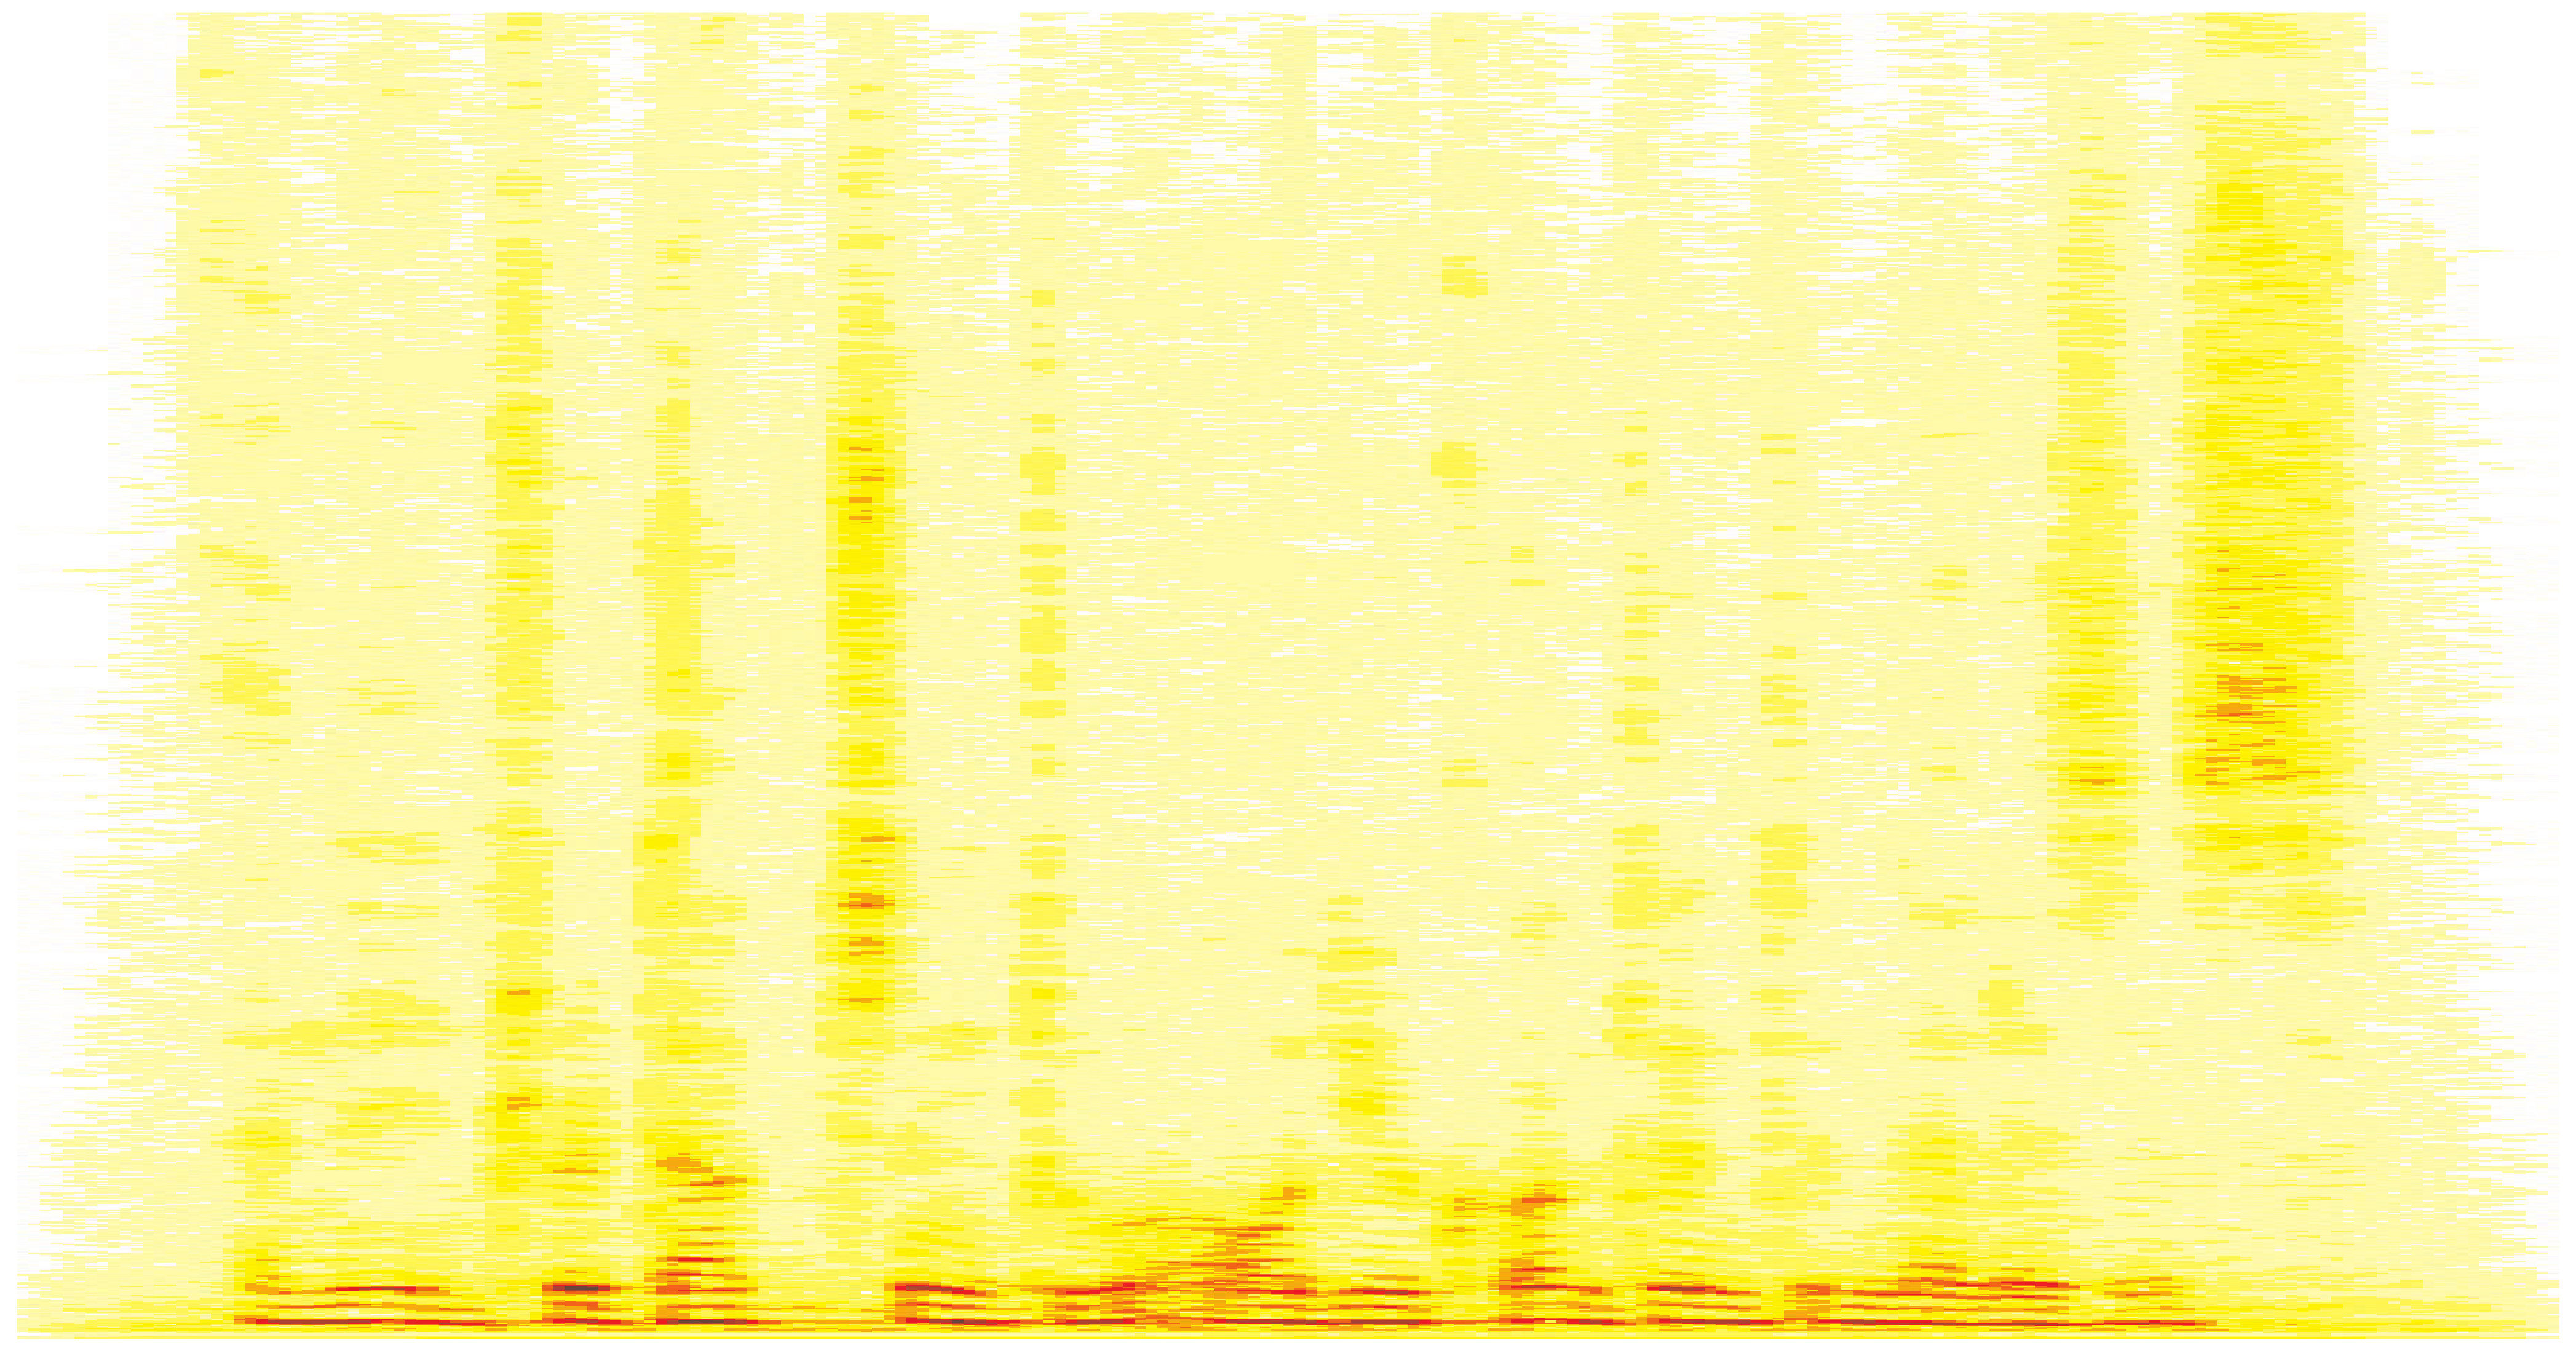
\includegraphics[width=\textwidth,height=3cm]{title}}

%%%%%%%%%%%%%%%%%%%%%%%%%%%%%%%%%%%%%%%%%%%%%%%%%%%%%%%%%%%%%%%%%%%%%%%%%%%%%%%%%%
%%%%%%%%%%%%%%%%%%%%%%%%%%%%%%%%%%%%%%%%%%%%%%%%%%%%%%%%%%%%%%%%%%%%%%%%%%%%%%%%%%
% colors
\definecolor{gtgold}{HTML}{E0AA0F} %{rgb}{0.88,0.66,1,0.06} [234, 170, 0]/256

%%%%%%%%%%%%%%%%%%%%%%%%%%%%%%%%%%%%%%%%%%%%%%%%%%%%%%%%%%%%%%%%%%%%%%%%%%%%%%%%%%
%%%%%%%%%%%%%%%%%%%%%%%%%%%%%%%%%%%%%%%%%%%%%%%%%%%%%%%%%%%%%%%%%%%%%%%%%%%%%%%%%%
% math
\DeclareMathOperator*{\argmax}{argmax}
\DeclareMathOperator*{\argmin}{argmin}
\DeclareMathOperator*{\atan}{atan}
\DeclareMathOperator*{\arcsinh}{arcsinh}
\DeclareMathOperator*{\sign}{sign}
\DeclareMathOperator*{\tcdf}{tcdf}
\DeclareMathOperator*{\si}{sinc}
\DeclareMathOperator*{\princarg}{princarg}
\DeclareMathOperator*{\arccosh}{arccosh}
\DeclareMathOperator*{\hwr}{HWR}
\DeclareMathOperator*{\flip}{flip}
\DeclareMathOperator*{\sinc}{sinc}
\DeclareMathOperator*{\floor}{floor}
\newcommand{\e}{{e}}
\newcommand{\jom}{\mathrm{j}\omega}
\newcommand{\jOm}{\mathrm{j}\Omega}
\newcommand   {\mat}[1]    		{\boldsymbol{\uppercase{#1}}}		%bold
\renewcommand {\vec}[1]    		{\boldsymbol{\lowercase{#1}}}		%bold

%%%%%%%%%%%%%%%%%%%%%%%%%%%%%%%%%%%%%%%%%%%%%%%%%%%%%%%%%%%%%%%%%%%%%%%%%%%%%%%%%%
%%%%%%%%%%%%%%%%%%%%%%%%%%%%%%%%%%%%%%%%%%%%%%%%%%%%%%%%%%%%%%%%%%%%%%%%%%%%%%%%%%
% media9
\newcommand{\includeaudio}[1]{{\includemedia[
                        addresource=audio/#1.mp3,
                        width=5mm,
                        height=5mm,
                        activate=onclick,
                        flashvars={
                            source=audio/#1.mp3  
                            &autoPlay=true
                        }]
                        {
\includegraphics[width=5mm, height=5mm]{SpeakerIcon}}
                        {APlayer.swf}}}
\newcommand{\audioautoplay}[1]{{\begin{center}\includemedia[
                            addresource=audio/#1.mp3,
                            width=.1\linewidth,
                            height=.01\linewidth,
                            activate=pageopen,
                            flashvars={
                                source=audio/#1.mp3  
                                &autoPlay=true
                            }]
                            {}
                            {APlayer.swf}\end{center}}}

\newcommand{\includevideo}[1]{{\begin{center}\includemedia[
                        addresource=video/#1.mp4,
                        width=0.8\linewidth,
                        height=0.4\linewidth,
                        activate=onclick,
                        flashvars={
                            source=video/#1.mp4  
                            &autoPlay=true
                        }]
                        {}
                        {VPlayer.swf}\end{center}}}
\newcommand{\videowithmatlab}[1]{{\begin{center}\includemedia[
                        addresource=video/animate#1.mp4,
                        width=0.8\linewidth,
                        height=0.4\linewidth,
                        activate=onclick,
                        flashvars={
                            source=video/animate#1.mp4  
                            &autoPlay=true
                        }]
                        {}
                        {VPlayer.swf}\end{center}\addreference{matlab source: matlab/animate#1.m}}}
                        

%%%%%%%%%%%%%%%%%%%%%%%%%%%%%%%%%%%%%%%%%%%%%%%%%%%%%%%%%%%%%%%%%%%%%%%%%%%%%%%%%%
%%%%%%%%%%%%%%%%%%%%%%%%%%%%%%%%%%%%%%%%%%%%%%%%%%%%%%%%%%%%%%%%%%%%%%%%%%%%%%%%%%
% other commands
\newcommand{\question}[1]{%\vspace{-4mm}
                          \setbeamercovered{invisible}
                          \begin{columns}[T]
                            \column{.8\textwidth}
                                \textbf{#1}
                            \column{.2\textwidth}
                                \vspace{-8mm}
                                \begin{flushright}
                                     
\includegraphics[scale=.5]{question_mark}
                                \end{flushright}
                                \vspace{6mm}
                          \end{columns}\pause\vspace{-12mm}}

\newcommand{\toremember}[1]{%\vspace{-4mm}
                          \begin{columns}[T]
                            \column{.8\textwidth}
                                \textbf{#1}
                            \column{.2\textwidth}
                                \vspace{-4mm}
                                \begin{flushright}
                                     
\includegraphics[scale=.5]{exclamation_mark}
                                \end{flushright}
                                \vspace{6mm}
                          \end{columns}\vspace{-6mm}}

\newcommand{\matlabexercise}[1]{%\vspace{-4mm}
                          \setbeamercovered{invisible}
                          \begin{columns}[T]
                            \column{.8\textwidth}
                                \textbf{matlab exercise}: #1
                            \column{.2\textwidth}
                                \begin{flushright}
                                     
\includegraphics[scale=.5]{logo_matlab}
                                \end{flushright}
                                %\vspace{6mm}
                          \end{columns}}

\newcommand{\addreference}[1]{  
                  
                    \begin{textblock*}{\baselineskip }(1.12\textwidth,.3\textheight) %(1.15\textwidth,.4\textheight)
                        \rotatebox{90}{\tiny {#1}}
                    \end{textblock*}}
                    
\newcommand{\figwithmatlab}[1]{
                    \begin{figure}
                        \centering
                        \includegraphics{#1}
                        %\label{fig:#1}
                    \end{figure}
                    
                    \addreference{matlab source: \href{https://github.com/alexanderlerch/ACA-Slides/blob/master/matlab/display#1.m}{matlab/display#1.m}}}
\newcommand{\figwithref}[2]{
                    \begin{figure}
                        \centering
                        \includegraphics{#1}
                        \label{fig:#1}
                    \end{figure}
                    
                    \addreference{#2}}  
                                    
\newcommand{\inserticon}[1]{

                    \begin{textblock*}{100mm}(14.5cm,7.5cm)
                        \includegraphics[height=.8cm,keepaspectratio]{#1}
                    \end{textblock*}}            

%%%%%%%%%%%%%%%%%%%%%%%%%%%%%%%%%%%%%%%%%%%%%%%%%%%%%%%%%%%%%%%%%%%%%%%%%%%%%%%%%%
%%%%%%%%%%%%%%%%%%%%%%%%%%%%%%%%%%%%%%%%%%%%%%%%%%%%%%%%%%%%%%%%%%%%%%%%%%%%%%%%%%
% counters
\newcounter{i}
\newcounter{j}
\newcounter{iXOffset}
\newcounter{iYOffset}
\newcounter{iXBlockSize}
\newcounter{iYBlockSize}
\newcounter{iYBlockSizeDiv2}
\newcounter{iDistance}



\subtitle{Module 8.3: Mood Recognition}

%%%%%%%%%%%%%%%%%%%%%%%%%%%%%%%%%%%%%%%%%%%%%%%%%%%%%%%%%%%%%%%%%%%%%%%%%%%%
\begin{document}
    % generate title page
	

\begin{frame}
    \titlepage
    %\vspace{-5mm}
    \begin{flushright}
        \href{http://www.gtcmt.gatech.edu}{\includegraphics[height=.8cm,keepaspectratio]{logo_GTCMT_black}}
    \end{flushright}
\end{frame}


    \section[overview]{lecture overview}
        \begin{frame}{introduction}{overview}
            \begin{block}{corresponding textbook section}
                    \href{http://ieeexplore.ieee.org/xpl/articleDetails.jsp?arnumber=6331125}{Chapter 8: Musical Genre, Similarity, and Mood} (pp.~158--161)
            \end{block}

            \begin{itemize}
                \item   \textbf{lecture content}
                    \begin{itemize}
                        \item   introduction to emotion and mood
                        \item   models for mood
                        \item   linear regression
                    \end{itemize}
                \bigskip
                \item<2->   \textbf{learning objectives}
                    \begin{itemize}
                        \item   describe Russel's arousal-valence plane
                        \item   discuss commonalities and differences between mood recognition and genre classification
                        \item   implement linear regression in Matlab
                    \end{itemize}
            \end{itemize}
            \inserticon{directions}
        \end{frame}

    \section[intro]{introduction}
        \begin{frame}{mood recognition}{introduction}
            
            \begin{itemize}
                \item	\textbf{objective}:identify mood/emotion of a song
                \item<2->   \textbf{terminology}:
                    \begin{itemize}
                        \item \textit{Music Mood Recognition} and \textit{Music Emotion Recognition} usually used synonymously
                    \end{itemize}
                \bigskip
                \item<3->   \textbf{processing steps} (similar to genre and similarity tasks)
                    \begin{itemize}
                        \item   extract features
                        \item   classify (possibly regression)
                    \end{itemize}
            \end{itemize}
        \end{frame}
   
    \section[mood]{mood \& emotion}
        \begin{frame}{mood recognition}{challenges}
            \question{What is the difference between \textit{mood} and \textit{emotion}}
            \begin{itemize}
                \item	\textit{emotion}: 
                    \begin{itemize}
                        \item   temporary, evanescent
                        \item   (directly) related to external stimuli
                    \end{itemize}
                \item	\textit{mood}: 
                    \begin{itemize}
                        \item   longer term, stable
                        \item   diffuse affect state
                    \end{itemize}
            \end{itemize}
        \end{frame}
            
        \begin{frame}{mood recognition}{challenges}
            \begin{itemize}
                \item   \textbf{ground truth data}
                    \begin{itemize}
                        \item   \textit{verbalization} of emotions/moods usually misleading
                        \item   not easily \textit{quantifiable}/categorizable
                        \item   change over time?
                    \end{itemize}
                \bigskip
                \item   \textbf{research focus}
                    \begin{itemize}
                        \item<2->	are established \textit{basic emotions} (happiness, anger, fear, \ldots) representative for music perception
                        \item<3->	\textit{aroused vs.\ transported} moods?
                    \end{itemize}
            \end{itemize}
        \end{frame}
                
    \section[models]{mood models}
        \begin{frame}{mood recognition}{models}
            \vspace{-3mm}
            \begin{itemize}
                \item	classification into \textbf{label clusters}\footfullcite{hu_exploring_2007}
                
                    \only<1>{
                    \begin{scriptsize}
                    \begin{tabular}{ccccc}
                        \\ \hline
                        \bf{\emph{Cluster 1}}	 & \bf{\emph{Cluster 2}}	 & \bf{\emph{Cluster 3}}	 & \bf{\emph{Cluster 4}}	 & \bf{\emph{Cluster 5}}\\ 
                         \hline
                        \bf{\textnormal{Rowdy}}	 & Amiable/Good Natured	 & Literate	 & Witty	 & Volatile\\
                        \bf{\textnormal{Rousing}}	 & Sweet	 & Wistful	 & Humorous	 & Fiery\\
                        \bf{\textnormal{Confident}}	 & Fun	 & Bittersweet	 & Whimsical	 & Visceral\\
                        \bf{\textnormal{Boisterous}}	 & Rollicking	 & Autumnal	 & Wry	 & Aggressive\\
                        \bf{\textnormal{Passionate}}	 & Cheerful	 & Brooding	 & Campy	 & Tense/Anxious\\
                        \bf{}	 & 	 & Poignant	 & Quirky	 & Intense\\
                        \bf{}	 & 	 & 	 & Silly	 & \\
                    \end{tabular}
                    \end{scriptsize}
                    }
                \item<2->	\textbf{mood model}, circumplex model\footfullcite{russel_circumplex_1980}
                    \only<2>{
                    \begin{figure}
                        \centering
                            \includegraphics[scale=.25]{graph/circumplex_affect}
                    \end{figure}
                    }
            \end{itemize}
        \end{frame}
    \section{regression}
        \begin{frame}{mood recognition}{mood model: regression modeling}
            \begin{itemize}
                \item   \textbf{mapping} 
                    \begin{itemize}
                        \item (N-dimensional) observation (feature) to 2-dimensional coordinate (valence/arousal)
                    \end{itemize}
                \bigskip
                \item   \textbf{training}
                    \begin{itemize}
                        \item find model to minimize error between data points and ``prediction''
                    \end{itemize}
            \end{itemize}
        \end{frame}
                
        \begin{frame}{linear regression}{introduction to regression 1/2}
                    \begin{itemize}
                        \item fit a linear function to a series of points  $(x_j,y_j)$
                            \begin{equation*}
                                y_n = m\cdot x_n + b
                            \end{equation*}
                    \end{itemize}
                \figwithref{LinearRegression}{\url{https://en.wikipedia.org/wiki/Linear_regression}}
        \end{frame}
                
        \begin{frame}{linear regression}{introduction to regression 2/2}
            \begin{itemize}
                \item   minimize error between model and data (here: least squares)
            \end{itemize}
            \begin{scriptsize}
            \begin{eqnarray*}
                e_n^2 &=& (y_n - mx_n - b)^2\\
                E &=& \sum (y_n - mx_n - b)^2\\
            \end{eqnarray*}
            \vspace{-10mm}
            \begin{columns}[T]
                \column{.5\linewidth}
                    \begin{eqnarray*}
                        \visible<2->{\frac{\partial E}{\partial b} = \sum -2(y_n - mx_n - b) &=& 0}\\
                        \visible<3->{-2\sum y_n +2\sum mx_n +2\sum b &=& 0}\\
                        \visible<4->{\sum mx_n + \sum b &=& \sum y_n}\\
                        \visible<5->{m\sum x_n + \mathcal{N}b &=& \sum y_n}
                    \end{eqnarray*}
                \column{.5\linewidth}
                    \begin{eqnarray*}
                        \visible<2->{\frac{\partial E}{\partial m} = \sum -2x_n(y_n - mx_n - b) =& 0&}\\
                        \visible<3->{-2\sum x_ny_n +2\sum mx_n^2 +2\sum bx_n =& 0&}\\
                        \visible<4->{\sum mx_n^2 + \sum bx_n = \sum x_ny_n&&}\\
                        \visible<5->{m\sum x_n^2 + b\sum x_n = \sum x_ny_n&&}
                    \end{eqnarray*}
            \end{columns}
            \bigskip
            \visible<6>{
            \begin{eqnarray*}
                &\Rightarrow&\\
                m &=& \frac{\mathcal{N}\sum x_ny_n-\sum x_n\sum y_n}{\mathcal{N}\sum x_n^2 -\left(\sum x_n\right)^2}\\
                b &=& \frac{\sum y_n}{\mathcal{N}}-m\frac{\sum x_n}{\mathcal{N}}\\
            \end{eqnarray*}
            }
            \end{scriptsize}
        \end{frame}
    \section{results}
        \begin{frame}{mood recognition}{range of results}
            \begin{itemize}
                \item   highly dependent on data
                \pause
                \item	\textbf{5 mood clusters}:\\ 40--60\% classification rate
                \bigskip
                \item	\textbf{mood model}:\\ 0.1--0.4 absolute prediction error (unit circle)
            \end{itemize}
        \end{frame}
    
    \section{summary}
        \begin{frame}{summary}{lecture content}
            \begin{itemize}
                \item   \textbf{emotion and mood}
                    \begin{itemize}
                        \item   emotion: temporary, related to external stimuli
                        \item   mood: long term, diffuse affective state
                    \end{itemize}
                \bigskip
                \item   \textbf{features}
                    \begin{enumerate}
                        \item   baseline features are identical to genre and similarity tasks
                    \end{enumerate}
                \bigskip
                \item   \textbf{inference}
                    \begin{enumerate}
                        \item   often done as regression (as opposed to classification)
                    \end{enumerate}
            \end{itemize}
            \inserticon{summary}
        \end{frame}
\end{document}
